% Chapter 1

\chapter{Introduction} % Main chapter title
\label{Chapter1} % For referencing the chapter elsewhere, use \ref{Chapter1} 

\lhead{Chapter 1. \emph{Introduction}} % This is for the header on each page - perhaps a shortened title

%----------------------------------------------------------------------------------------
% Section - Context
%----------------------------------------------------------------------------------------

\section{Context}

%-- machine learning in safety-critical systems
\Gls{ml} algorithms are becoming increasingly present in systems that operate within shared environments
with humans, or involve direct interaction with humans themselves~\citep{pereira}. These systems 
are often defined as safety-critical, such that their failures lead to unintended and potentially harmful behaviours~\citep{amodei}.
Examples of these systems include autonomous automotive systems, traffic control systems, medical devices, aviation software,
industrial robotics, and many more cyber-physical systems that interact with our environment.
Many of these systems have so far only existed as proof of concepts, but are steadily approaching commercial use within our society.

%-- prone to adversarial attacks
Additionally, recent research has exposed broad vulnerabilities to adversarial attacks within data driven \gls{ml} algorithms,
including \Glspl{nn}; where applying small but intentional perturbations to an input which are not noticible to humans,
can lead to a model outputting an incorrect classification with high confidence~\citep{goodfellow}.
An example of such an attack can be seen in \textit{Fig.~\ref{fig:adversarialpatch}}.
Consequently, the testing and verification of \gls{ml} for the use of controlling safety-critical systems has become a focused area of research in recent years.

\begin{figure}[H]
	\centering
        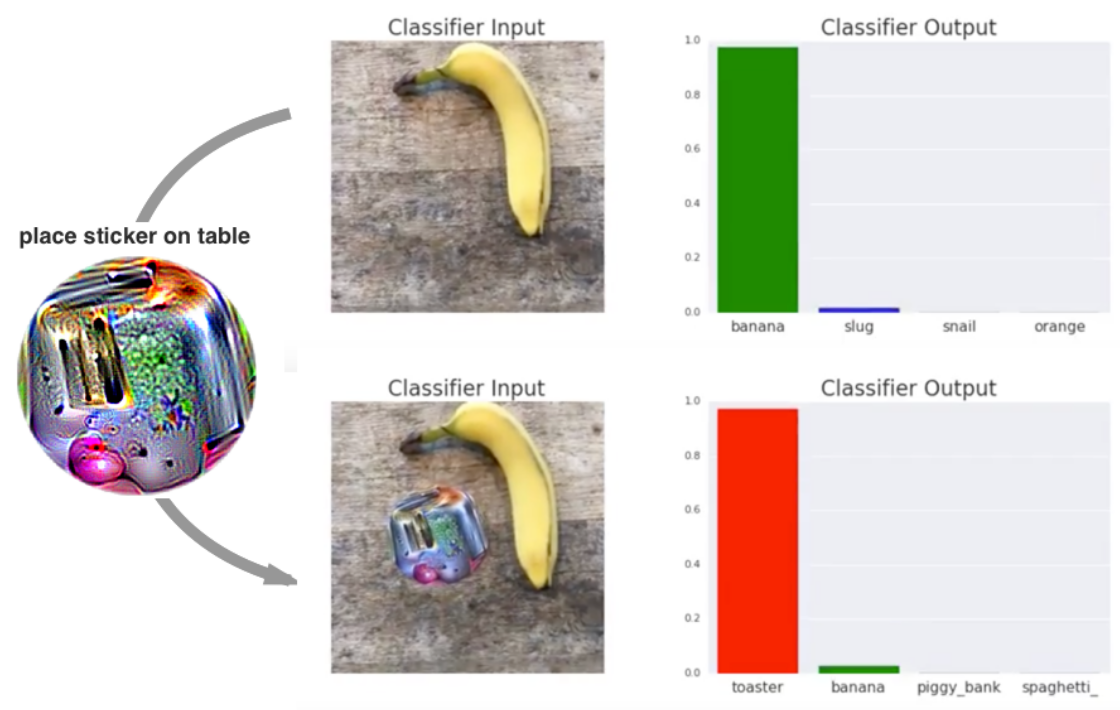
\includegraphics[width=0.8\textwidth]{media/introduction/sticker.png}
        \rule{35em}{0.5pt}
        \caption[Google's adversarial patch]{\textbf{Google's Adversarial Patch} -- An example of a method to create targeted adversarial attacks on \glspl{nn} by adding carefully designed noise via a physical patch~\citep{brown2018}.}\label{fig:adversarialpatch}
\end{figure}

%-- definition of software testing and verification
This thesis will use the following definitions for software \textit{testing} and \textit{verification}.
Software testing, or validation, is defined as the evaluation of a system under various conditions and observing its behaviour while
looking for defects~\citep{pereira}. In the context of \gls{ml} development, testing is used to
ensure that a trained model generalises accurately to some previously unseen test data.

Verification is defined as the process of determining whether the products of a phase of the software development process fulfill
the requirements established during the previous phase~\citep{ammann2008}. Formal verification in other words, formulates logical arguments
that a system will not act abnormally under a wide range of circumstances, and can be used to determine not only generality, but also the robustness and correctness of a system.

%-- challenges when verifying ML systems
The challenges regarding verification of \gls{ml} models stem from the typically lower interpretability and more statistically-oriented nature of their algorithms, which
lead to a lower degree of understanding than software that is explicitly programmed to perform a specific task~\citep{bishop}. These types of systems are
commonly referred to as \textit{black box} systems, where the internal mechanisms are not revealed; in other words, it is impossible to understand a model just by
looking at its parameters~\citep{molnar2019}.

%----------------------------------------------------------------------------------------
% Section - Motivation
%----------------------------------------------------------------------------------------
\section{Motivation}

Public calls for \textit{sensible} or \textit{verifiable \Gls{ai}} have been raised in recent years due to ever increasing
development of complex and pervasive systems that are entering into our everyday lives~\citep{russell2016}.

Formal verification of software systems has seen significant progress since the early
verification systems. These early systems~\citep{polak1979, boyer1990, guaspari1993} often struggled to be 
widely adopted into industry applications. However, due to the ever increasing complexity of deployed
software, new verification tools have been developed with the intent of being accessible to a wide range
of industry software engineers~\citep{fisher2017}.

On the other hand, verification of \gls{ml} systems has 
seen relatively little progress, with the exception of \Glspl{mas}~\citep{lomuscio2017, kouvaros2016}.
Indeed, due to the nature of \gls{aiv} research, there are limited 
programming tools available for researchers in this area. This is especially true for work
within \gls{ml}, as the programming languages and tools commonly used for \textit{traditional} verifcation are often
disparate from those widely adopted by the \gls{ml} communities. 

%-- ml languages
Popular programming languages used for \gls{ml} such as Python or Matlab currently have comparitively less
formal verification tools available than those concerned with system infrastructure or embedded applications.
Additionally, \gls{aiv} toolkits for \gls{ml} tasks in these languages are still in early stages of development, and mainly focused
on the verification of \glspl{nn}~\citep{kokke2020}. 

%-- programming languages are forever changing
Furthermore, the landscape of \gls{ml} programming itself is forever shifting, and while there is not yet a programming 
language dedicated for \gls{ml} tasks, huge efforts from programming language designers have been made 
in developing \gls{ml} libraries for existing languages. This is necessary in order to handle the 
extremely high computational demands, and to simplify 
model languages to make them easier to add domain-specific optimisations and features~\citep{innes2017}.

%- GO

A prime example of such development can be seen in the Go programming language, or \textit{GoLang}. A relatively new language, which was originally developed by Google in 2009 with the intention
of creating a modern general-purpose language similar to C. 
GoLang has seen a surge in popularity within the \gls{ml} community since
the release of its first extensive \gls{ml} package, \textit{Gorgonia}, in 2016, which heavily relies on the use of expression graphs~\citep{chew2016}.
This package allows GoLang developers
to take advantage of automatic and symbolic differentiation, gradient descent optimisations, numerical stabilisation,
added support for CUDA/GPGPU computation, and comparatively quicker speeds than its Python counterparts (Theano and TensorFlow)~\citep{golang2020}.

% -- TODO | discuss Microsoft's efforts in F (as annotated by Katya)
A good example of a programming paradigm shift towards dedicated \gls{ml} languages, is Microsoft's efforts in developing
an efficient differentiable version of the \Gls{fp} language F~\citep{shaikhha2019}.

%-- need for aiv development in other languages
Consequently, as programming languages continue to develop \gls{ml} capabilities, there is a need for 
exploring new and scalable approaches for developing \gls{aiv} tools in these languages.
This is especially important for programming languages which are being adopted by industry to implement \gls{ml} models
for the use within safety-critical or pervasive systems.

%----------------------------------------------------------------------------------------
% Section 3
%----------------------------------------------------------------------------------------
\section{Aims \& Objectives}

%-- aims
% explore the methods for efficiently implementing formal verification tools in a wide range of
% programming languages used for machine learning

% Investigate different approaches for implementing formal verification tools in a wide range of programming
% languages used for \gls{ml}

%-- talk about go, and machine learning

%- Go safety critical applications

%- aim

The aim of this project is to investigate the current programming paradigms within \gls{ml} development,
and to explore the suitability of current formal verification toolkits available to them. Subsequently,
this thesis will aim to design and implement a GoLang formal methods framework for Gorgonia \glspl{nn},
providing GoLang \gls{ml} developers with a set of tools which will allow them to produce safe and
fair \gls{ai} applications.

This framework will extend upon the work made by~\citep{kokke2020}, and the Sapphire library implemented in Python
which successfully translates TensorFlow feed-forward \gls{nn} model queries to the Z3 \Gls{smt} solver created by Microsoft Research~\citep{demoura2008}.

% - objective

% To achieve this, the primary objective is to implement a GoLang package which allows the binding of Gorgonia \gls{nn} models to
% Z3 SMT solvers. Similar to the Sapphire library written in Python~\citep{kokke2020}.

To achieve this project's aims, the following objectives should be met:

\begin{itemize}
    \setlength\itemsep{0em}
    \item \textit{Objective 1 -} Conduct a feasibility study with regards to developing a formal methods framework for \glspl{nn} in Go.
    \item \textit{Objective 2 -} Implement bindings that map the parameters of a Gorgonia \gls{nn} model to
        Z3 variables.
    \item \textit{Objective 3 -} Select example training data sets in order to train and verify \gls{nn} models using this project's formal methods framework.
    \item \textit{Objective 4 -} Implement a series of \gls{nn} models in Gorgonia using the data sets mentioned in \textit{Objective 3}.
    \item \textit{Objective 5 -} Verify the correctness of Gorgonia \glspl{nn} using the bindings developed in \textit{Objective 2}.
    \item \textit{Objective 6 -} Make conclusions about the developed framework's benefits and limitations, and discuss future improvements to the methodology as described in \textit{Objective 1}.
\end{itemize}
